\documentclass{article}
\usepackage[margin=2.5cm, includefoot, footskip=30pt]{geometry}

\setlength{\parindent}{0em}
\setlength{\parskip}{1em}
\renewcommand{\baselinestretch}{1}

%%%%Packages%%%%
\usepackage{amsmath}
\usepackage{booktabs}
\usepackage{graphics}
\usepackage{multicol}
\usepackage[ruled,vlined]{algorithm2e}
\usepackage{setspace}
\usepackage{graphicx}
\usepackage{subcaption}
\usepackage{hyperref}
\usepackage{color,colortbl}
\usepackage{array}
\usepackage{booktabs}
\usepackage{tabularx}
\usepackage{wrapfig, blindtext}
%%%%%%%%%%%%%%%%%

\definecolor{Gray}{gray}{0.92}
\usepackage[first=0,last=9]{lcg}
\newcommand{\ra}{\rand0.\arabic{rand}}

\setlength{\tabcolsep}{3pt}

\title{A meta analysis of tournaments and an evaluation of performance in the
Iterated Prisoner's Dilemma.}
\author{Nikoleta E. Glynatsi, Dr Vincent A. Knight}
\date{}

\begin{document}

\maketitle

\begin{abstract}

The iterated prisoner's dilemma has been used for decades as a powerful model of
behavioural interactions. From the celebrated performance of Tit for Tat, to the
introduction of the zero-determinant family, to the use of sophisticated
strategies such as neural networks, the literature has been exploring the
performance of strategies in the game for years. Most of these strategies
are now accessible due to an open source package. This manuscript make use
of the open source and it's strategy data base to a conducts a meta analysis of
iterated prisoner's dilemma tournaments. The aim is to evaluate the performance
of these strategies and finally answer the question: which is the best strategy
in the game?
\end{abstract}

\section{Background}

The iterated prisoner's dilemma is a repeated two player game that models
situations in which self-interest clashes with collective interest. At each turn,
the players simultaneously and independently make a choice between cooperation (C) and
defection (D) whilst their prior interactions matter. The payoffs at each given turn are defined by the matrix,

\[\begin{pmatrix}
R & S \\
T & P
\end{pmatrix}\]

where \(T > R > P > S\) and \(2R > T + S\). The most common values used in
the literature, and in this paper, are $R=3, P=1, T=5, S=0$.

Since the computer tournaments of R. Axelrod in 1980s several academic papers
are published in the field regarding the performance of strategies in the
iterated prisoner's dilemma. In the 80's following the strong performance of Tit For Tat
in both Axelrod's computer tournaments~\cite{Axelrod1980a, Axelrod1980b}, and
moreover in a series of evolutionary experiments~\cite{Axelrod1981}, the strategy
was thought as the most robust basic strategy in the iterated prisoner's
dilemma. However, the strategy's poor performance in environments with
noise~\cite{Bendor1991, Donninger1986, Molander1985, Hammerstein1984},
made room for other protagonists, such as, Nice and Forgiving~\cite{Bendor1991},
Pavlov~\cite{Nowak1993} and Generous Tit For Tat~\cite{Nowak1992}.

Yet again, in 2012 another set of strategies was introduced as the dominant set
of strategies~\cite{Press2012}. These were called zero-determinant strategies,
and by forcing a linear relationship between the payoffs they can ensure that
they will never receive less than their opponents. However, in~\cite{Harper2017}
a tournament containing over 200 strategies, including the zero-determinant strategies
introduced in~\cite{Press2012}, was performed and none of the zero-determinant
strategies ranked in top spots. Instead, the top ranked strategies were a set of
trained strategies based lookup tables, hidden markov models and finite state
automata.
%TODO reference the archetypes of the archetypes used the IPD?

Thus, the following question is raised here: which are the true dominant
strategies in the iterated prisoner's dilemma?

This manuscript uses the open source package
Axelrod-Python~\cite{axelrodproject} to simulate a large number of computer
tournaments using as many strategies as possible from the literature. The aim is
evaluate the performance of these strategies in a tournament and futhermore,
explore the factors of their success. This is done not for standard round robin
tournaments, but also for noisy, probabilistic ending and noisy probabilistic
ending tournaments.

The structure of this manuscript is as follows. In
Section~\ref{section:data_collection} the data collection is covered. In
Section~\ref{section:top_performances}, the best performed strategies for each
type of tournament and overall are presented.
Section~\ref{section:evaluation_of_performance}, explores the traits which
contribute to good performance and finally in Section~\ref{section:conclusion}
we conclude and summarise the results.

\section{Data generating process}\label{section:data_collection}

For the purposes of this manuscript a data set containing results on iterate
prisoner's dilemma tournaments has been generated, which is available at. This
was done using the open source package Axelrod-Python~\cite{axelrodproject},
more specifically, version 3.0.0. Axelrod-Python allows for different types of
iterated prisoner's dilemma computer tournaments to be simulated whilst
containing a list of over 190 strategies. Most of these are strategies described
in the literature with a few exceptions being strategies that have been
contributed specifically to the package. Though Axelrod-Python features several
tournament types, this work considers only standard, noisy, probabilistic ending
and noisy probabilistic ending tournaments.

\textbf{Standard tournaments}, are tournaments similar to that of Axelrod's
in~\cite{Axelrod1980a}. There are \(N\) strategies which all play an iterated
game of \(n\) number of turns against each other. Note that self interactions and
a match against a random strategy are not included. Similarly, \textbf{noisy tournaments}
have \(N\) strategies and \(n\) number of turns but at each turn there is a
probability \(p\) that a player's action will be flipped.
\textbf{Probabilistic ending tournaments}, are of size \(N\) and after each turn
a match between strategies ends with a given probability \(e\). Finally,
\textbf{noisy probabilistic ending} tournaments have both a noise probability
\(p\) and an ending probability \(e\). For smoothing the simulated results a
tournament is repeated for \(r\) number of times and the ranks are based on the
average score a strategy achieved and not by number of wins. A summary of
each tournaments' parameters is given in Table~\ref{table:tournaments_parameters}.

\begin{table}[!htbp]
    \begin{center}
        \resizebox{.85\textwidth}{!}{
        \begin{tabular}{lccccc}
    \toprule
    tournament type & number of strategies & turns & noise probability & probability of match ending \\
    \midrule
    standard & $N$  & $n$ & - & - \\
    noisy & $N$  & $n$ & $p$ & - \\
    probabilistic ending & $N$  & - & - & $e$ \\
    noisy probabilistic ending & $N$  & - & $p$ & $e$ \\
    \bottomrule
        \end{tabular}}
    \end{center}
    \caption{Tournament types' parameters.}
    \label{table:tournaments_parameters}
\end{table}

The process of generating data implemented in this manuscript is given by
Algorithm~\ref{algorithm:data_generation}. For each trial a random
size \(N\) is selected, and from the list of 195 strategies
in~\cite{axelrodproject}, a random list of \(N\) strategies is chosen. For the
given list of strategies a standard, noise, probabilistic ending and a noisy
probabilistic ending tournament are performed and repeated \(r\) times.
The parameters for the tournaments as well as the number of repetitions are
selected once for each trial. The parameters and their respective minimum and
maximum values are given by Table~\ref{table:parameters_values}.

The source code for the data generating process as well as the source code for
the analysis which will be discussed in the following sections have been written
following best practices~\cite{Aberdour2007, Benureau2018}. It has been packaged
and is available here.

\begin{algorithm}[!htbp]
    \setstretch{1.35}
    \ForEach{\text{seed} $\in [0, 12285]$}{
        $N \gets \text{randomly select integer}\in [N_{min}, N_{max}]$\;
        $\text{players} \gets  \text{randomly select $N$ players}$\;
        $r \gets  \text{randomly select integer}\in [r_{min}, r_{max}]$\;
        $n \gets  \text{randomly select integer}\in [n_{min}, n_{max}]$\;
        $p \gets  \text{randomly select float}\in [p_{min}, p_{max}]$\;
        $e \gets   \text{randomly select float}\in [e_{min}, e_{max}]$\;
        \vspace{0.4cm}
        $\text{result standard}$ $\gets$ Axelrod.tournament$(\text{players}, n, r)$\;
        $\text{result noisy}$ $\gets$ Axelrod.tournament$(\text{players}, n, p, r)$\;
        $\text{result probabilistic ending}$ $\gets$ Axelrod.tournament$(\text{players}, e, r)$\;
        $\text{result noisy probabilistic ending}$ $\gets$ Axelrod.tournament$(\text{players}, p, e, r)$\;

    }
    \KwRet{result standard, result noisy, result probabilistic ending,
    result noisy probabilistic ending}\;
    \caption{Data generating Algorithm}
    \label{algorithm:data_generation}
\end{algorithm}

\begin{table}[!htbp]
    \begin{center}
        \resizebox{.6\textwidth}{!}{
        \begin{tabular}{lcccc}
    \toprule
    parameter & parameter explanation &   min value & max value \\
    \midrule
    $N$ & number of strategies  & 3 & 195 \\
    $r$ & number of repetitions  & 10 & 100 \\
    $n$ & number of turns      & 1 & 200 \\
    $p$ & probability of flipping action at each turn  & 0 & 1   \\
    $e$ & probability of match ending in the next turn & 0 & 1   \\
    \bottomrule
        \end{tabular}}
    \end{center}
    \caption{Data generation parameters' values}
    \label{table:parameters_values}
\end{table}

A total of 12,285 trials of Algorithm~\ref{algorithm:data_generation} have been
performed. For each trial the results for 4 different tournaments were collected,
thus a total of 49,140 $(12,285 \times 4)$ tournament results have been
retrieved. Each tournament outputs a result summary in the form of
Table~\ref{table:output_result}. The result summary has a length \(N\) because
each row contains information for each strategy that participated in the tournament.
The information include the strategy's rank $(R)$, median score, the rate with
which the strategy cooperated $(C_r)$, it's wins and the probability that the strategy
cooperated in the opening move. Moreover the summary result includes the rates
of a strategy being in any of the four states ($CC, CD, DC, DD$), and the rate
of which the strategy cooperated after each state.

\newcolumntype{g}{>{\columncolor{Gray}}c}
\begin{table}[!htbp]
    \begin{center}
    \resizebox{\textwidth}{!}{
    \begin{tabular}{ccccccgcgcgcgcg}
    \toprule 
    & & & & & &   \multicolumn{8}{g}{Rates}  \\
    Rank $(R)$ & Name & Median score & Cooperation rating $(C_r)$ & Win & Initial C &
    CC & CD & DC & DD & CC to C & CD to C & DC to C & DD to C \\
    0 &  EvolvedLookerUp2 2 2 & 2.97 & 0.705 & 28.0 & 1.0 & 0.639 & 0.066 & 0.189 &
    0.106 & 0.836 & 0.481 & 0.568 & 0.8 \\
    1 &  Evolved FSM 16 Noise 05 & 2.875 & 0.697 & 21.0 & 1.0 & 0.676 & 
    0.020 & 0.135 & 0.168 & 0.985 & 0.571 & 0.392 & 0.07 \\
    2 & PSO Gambler 1 1 1 & 2.874 & 0.684 &  23.0 &     1.0 &    0.651 &    0.034 &    0.152 &    0.164
    & 1.000 & 0.283 & 0.000 & 0.136 \\
    3 &  PSO Gambler Mem1 &  2.861 &        0.706 &  23.0 &      1.0 &    0.663
    &    0.042 &    0.145 &    0.150 &  1.000 &  0.510 &  0.000 &  0.122 \\
    4 &          Winner12 &  2.835 &        0.682 &  20.0 &      1.0 &
    0.651 &    0.031 &    0.141 &    0.177 &  1.000 &  0.441 &  0.000 &  0.462 \\
    $\dots$ & $\dots$ & $\dots$ & $\dots$ & $\dots$ & $\dots$ & $\dots$ & $\dots$ &
    $\dots$ & $\dots$ & $\dots$ & $\dots$ & $\dots$ & $\dots$ \\
    \bottomrule
    \end{tabular}}
\end{center}
\caption{Output result.}\label{table:output_result}
\end{table}

Several other measures have been manually calculated/retrieved and have been
included in the data set. These include properties of the strategies as well as
measures regarding the tournament, such as the parameters of
Table~\ref{table:parameters_values}. All these measures are summarized and
described Table~\ref{table:manual_measures}.

\newcolumntype{g}{>{\columncolor{Gray}}c}
\begin{table}[h]
    \begin{center}
    \resizebox{\textwidth}{!}{
    \begin{tabular}{gcgcgc}
    \toprule
    measure & measure explanation &  source & value type & min value & max value \\
    \midrule
normalized rank $(r)$ & The rank of the strategy divided by the tournament size & result summary & float & 0 & 1 \\
memory depth &  Strategy's memory size & strategy classifier from~\cite{axelrodproject} & integer & 0 & $\infty$ \\
stochastic  &  If a strategy is stochastic & strategy classifier from~\cite{axelrodproject} & boolean  & False &  True \\
makes use of game &  If a strategy makes used of the game information & strategy classifier from~\cite{axelrodproject} & boolean  & False &  True \\
makes use of length &  If a strategy makes used of the number of turns & strategy classifier from~\cite{axelrodproject} & boolean  & False &  True \\
SSE & A measure of how far a strategy is from extortionate behaviour & method described in [ref] & float & 0 & 1 \\
max cooperating rate $(C_{\text{max}})$  & The biggest cooperating rate in the tournament & result summary & float & 0 & 1 \\
min cooperating rate $(C_{\text{min}})$ & The smallest cooperating rate in the tournament & result summary & float & 0 & 1 \\
median cooperating rate $(C_{\text{median}})$ & The median cooperating rate in the tournament & result summary & float & 0 & 1 \\
mean cooperating rate $(C_{\text{mean}})$ & The mean cooperating rate in the tournament & result summary & float & 0 & 1 \\
$C_r$ / $C_{\text{max}}$ & A strategy's cooperating rate divided by the maximum & manually & float & 0 & 1 \\
$C_r$ / $C_{\text{min}}$ & A strategy's cooperating rate divided by the minimum & manually & float & 0 & 1 \\
$C_r$ / $C_{\text{median}}$ & A strategy's cooperating rate divided by the median & manually & float & 0 & 1 \\
$C_r$ / $C_{\text{mean}}$ & A strategy's cooperating rate divided by the mean & manually & float & 0 & 1 \\
    \bottomrule
        \end{tabular}}
    \end{center}
    \caption{Manually calculated/retrieved measures.}
    \label{table:manual_measures}
    \end{table}

These measures will be used in more detail in the following sections.

% Might move these measures to the sections in which they are actual used as
% it feels like an overload of info in this section.

The data collection and the output from the generated tournaments have been
covered in this section. The measures that will be used in the analysis of the
following sections have been presented. These are also summarised in Table in
the Appendix. In the following Section, the top performances at each tournament
are overall are presented.

\section{Top ranked strategies}\label{section:top_performances}

This section evaluates the performance of 186 strategies. These can be find in
the Appendix. The performance of each strategy will be evaluated for each type
of tournament independently. In Section~\ref{subsection:standard_tournament} the
strategies are evaluated on their performance in standard tournaments, in
Section~\ref{subsection:noisy_tournament} in noisy, and the rest in
Sections~\ref{subsection:probend_tournament}
and~\ref{subsection:noisy_probend_tournament}.

Each tournament could have participated in multiple tournaments of the same
type. On average a strategy participated in 5690 different tournaments of each
type. For example Tit For Tat has participated in a total of 5569 standard
tournaments. The strategy's normalised ranks distribution is given in
Figure~\ref{fig:tit_for_tat_r_distribution}. As a result, of the multiple entries of
strategies their performance in this manuscript is evaluated based on the median
normalised rank denoted as \(\bar{r}\). Note that a value of \(\bar{r} = 0\)
means that a strategy the winner of the tournament where a value of \(\bar{r} = 1\)
means that the strategy came last.

\begin{figure}
    \centering
    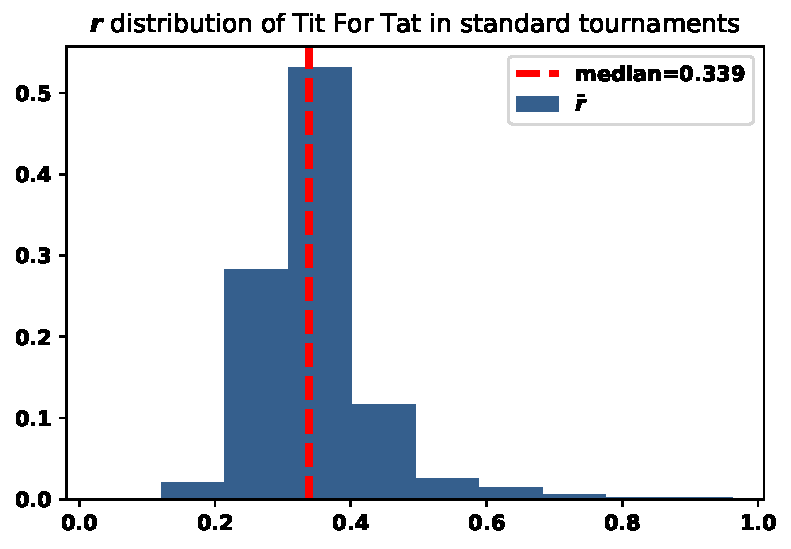
\includegraphics[width=.5\textwidth]{../images/tit_for_tat_r_distribution.pdf}
    \caption{Tit For Tat's $r$ distribution for standard tournaments.}
    \label{fig:tit_for_tat_r_distribution}
\end{figure}

Following the analysis of each tournament type, in Section~\ref{subsrction:overall}
the results are merged and the strategies are evaluated in their overall performances
over all the different tournaments.

\subsection{Standard tournaments}\label{subsection:standard_tournament}

The results presented in this section are based on $12,285$ different standard
tournaments. Each tournament has on average 122 participants, a length of
100 turns and was repeated 55 times.

The top 15 performances in standard tournaments are given by
Table~\ref{table:std_results}. The 10 out of the 15 are strategies introduced
in~\cite{Harper2017}. These have been trained using FSM (finite state automata),
HMM (hidden markov models), ANN (artificial neural networks), lookup tables
(LookerUp) and stochastic lookup tables (Gambler). Specifically, the have been
trained using the strategy list of~\cite{axelrodproject} in standard
tournaments. Thus their performance was to be expected. DoubleCrosser, and Fool
Me Once, are not from the literature but from~\cite{axelrodproject}.
DoubleCrosser is a strategy that makes use of the length of the match because is
set to defect on the last two rounds. The strategy is expected to not perform as
well in probabilistic ending tournaments. Finally, Winner 12~\cite{Mathieu2017}
and DBS are both from the the literature. DBS~\cite{Au2006} is strategy
specifically designed for noisy environments, however, it ranks highly only in
standard ones.

\begin{table}[!htbp]
    \centering
    \resizebox{.3\textwidth}{!}{
    \begin{tabular}{lr}
\toprule
{} &  $\bar{R}$ in standard tournaments \\
Name                    &                                    \\
\midrule
Evolved HMM 5           &                           0.006579 \\
Evolved FSM 16          &                           0.009901 \\
EvolvedLookerUp2\_2\_2    &                           0.010638 \\
Evolved FSM 16 Noise 05 &                           0.016393 \\
PSO Gambler 2\_2\_2       &                           0.021390 \\
Evolved ANN             &                           0.028736 \\
Evolved ANN 5           &                           0.033898 \\
PSO Gambler 1\_1\_1       &                           0.037234 \\
Evolved FSM 4           &                           0.048387 \\
PSO Gambler Mem1        &                           0.050000 \\
Winner12                &                           0.059459 \\
Fool Me Once            &                           0.061224 \\
DBS                     &                           0.070866 \\
DoubleCrosser           &                           0.071895 \\
BackStabber             &                           0.075000 \\
\bottomrule
\end{tabular}
}
    \caption{Standard top performances}\label{table:std_results}
\end{table}

The distributions of $\bar{r}$ for top ranked strategies are given in
Figure~\ref{fig:std_results}. The distributions are skewed towards zero and the
highest median is at 0.075. These strategies would mostly rank high when they
participated in a tournament. This is not true for the rest of the tournament
types. In the following sections $\bar{r}$ and subsequently the performances are
more variant.

\begin{figure}[!htbp]
    \centering
    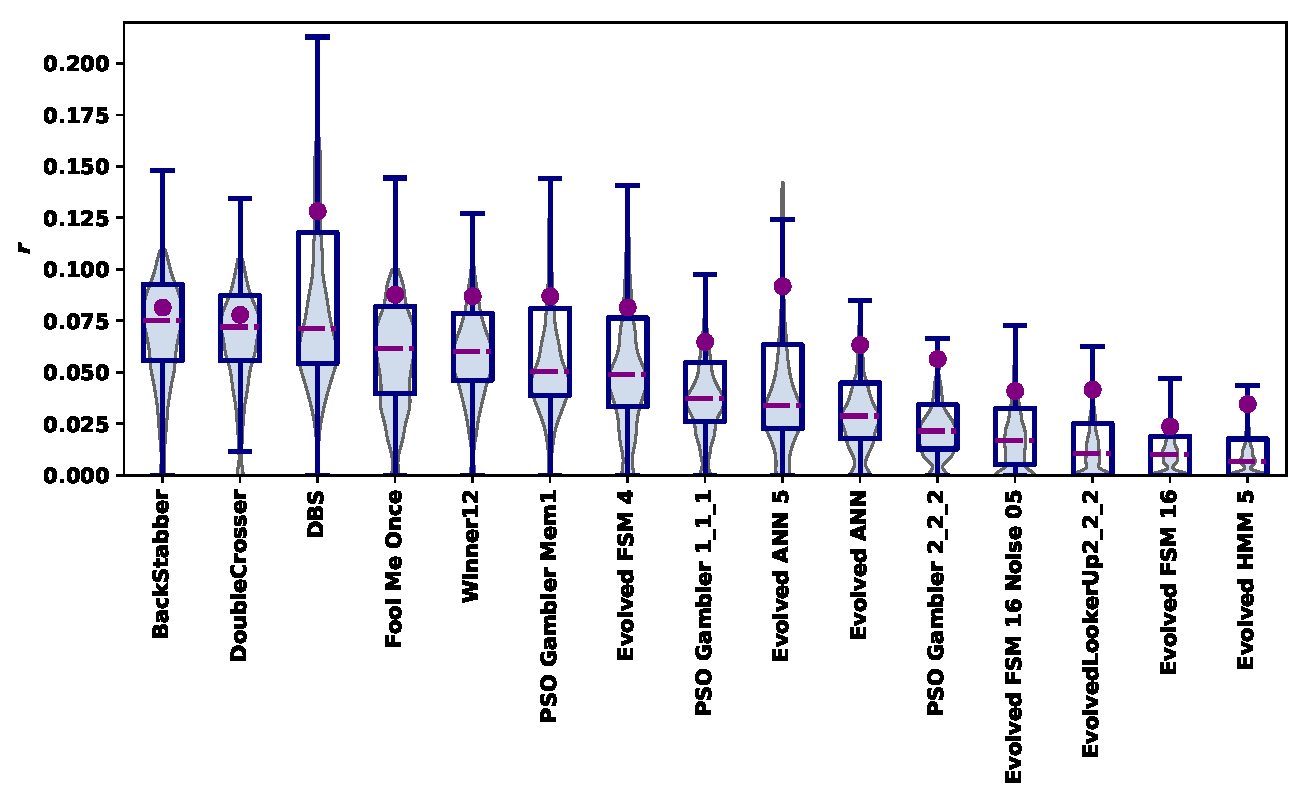
\includegraphics[width=.8\textwidth]{../images/performance_standard.pdf}
    \caption{$\bar{r}$ distributions of top 15 strategies.}\label{fig:std_results}
\end{figure}

\subsection{Noisy tournaments}\label{subsection:noisy_tournament}

Similarly to Section~\ref{subsection:standard_tournament} the results presented
here are based on $12,285$ different noisy tournaments. The strategies have been
ranked based on their \(\bar{r}\) and the top 15 are given by
Table~\ref{table:noisy_results}. The distributions of their corresponding
\(\bar{r}\) is also given by Figure~\ref{fig:noisy_results}.

The top strategies include two well known strategies Tit For 2
Tats~\cite{Axelrod1980b} and Hard Tit For 2 Tats~\cite{Stewart2012} which are
strategies that will defect only after the have received two defections from the
opponent. The Retaliate strategies are set of strategies from~\cite{axelrodproject}
that start by cooperating but will retaliate once the opponent's wins and
defections surpass a curtain threshold. Strategies ShortMem~\cite{Carvalho2013},
Grumpy, $e$ and $\phi$ are strategies that make decisions based on the
cooperations to defections. Cycler Hunter tries to extort strategies that play
cyclically and Risky QLearn uses a Q learning algorithm. Notably a very simple
strategy, Cooperator, has been ranked third.

\begin{table}[!htbp]
    \centering
    \resizebox{.28\textwidth}{!}{
    \begin{tabular}{lr}
\toprule
Name                &                        $\bar{r}$\\
\midrule
Grumpy              &                         0.13953 \\
$e$                 &                         0.19048 \\
Cooperator          &                         0.19565 \\
Tit For 2 Tats      &                         0.20520 \\
Cycle Hunter        &                         0.22222 \\
Risky QLearner      &                         0.22424 \\
Retaliate 3         &                         0.23077 \\
Retaliate 2         &                         0.23762 \\
Retaliate           &                         0.24309 \\
Hard Tit For 2 Tats &                         0.24658 \\
Limited Retaliate 3 &                         0.25000 \\
ShortMem            &                         0.25272 \\
Limited Retaliate   &                         0.25698 \\
Limited Retaliate 2 &                         0.26027 \\
$\phi $              &                         0.26201 \\
\bottomrule
\end{tabular}
}
    \caption{Noisy top performances}\label{table:noisy_results}
\end{table}

From Figure~\ref{fig:std_results} it is evident that the normalised rank distributions
in noisy environments are more variant and have higher median values compared
to standard tournament. Moreover, the distributions are skewed both towards
0 and 1 which indicate that the top ranked strategies ranked first and last
in several tournaments. However, the low values of the median shows that the
have won most of the tournaments.

\begin{figure}[!htbp]
    \centering
    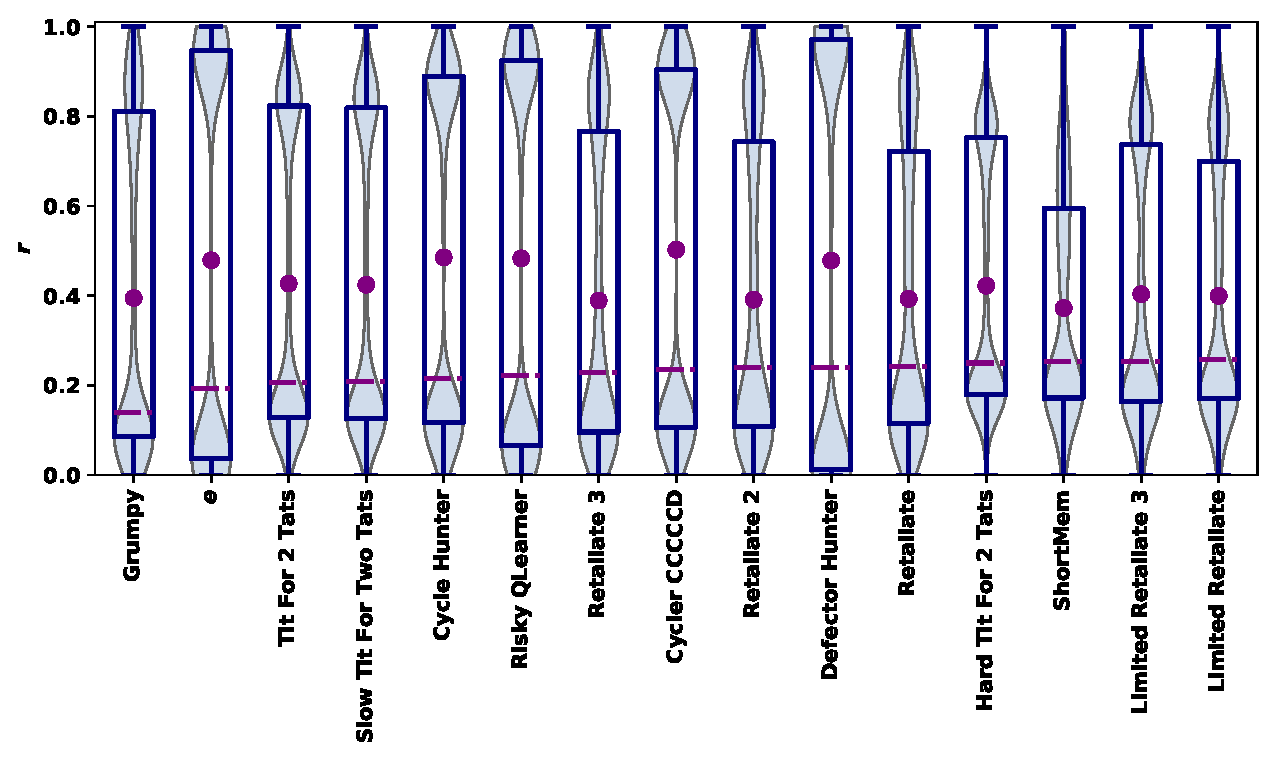
\includegraphics[width=.8\textwidth]{../images/performance_noise.pdf}
    \caption{\(\bar{r}\) distributions for best performed strategies in noisy tournaments.}
    \label{fig:noisy_results}
\end{figure}

\subsection{Probabilistic ending tournaments}\label{subsection:probend_tournament}

In this section the performances in probabilistic ending tournaments are discussed.
The 15 top ranked strategies are given by Table~\ref{table:prob_end_results}
and their respective $\bar{r}$ distributions in Figure~\ref{fig:probend_results}.

Fortress 3, Fortress 4 (both introduced in~\cite{Ashlock2006}),
Raider~\cite{Ashlock2014} and Solution B1~\cite{Ashlock2014} are strategies
based on finite state automata introduced by Daniel and Wendy Ashlock. These
strategies have been evolved using reinformed learning. However, there were
trained to maximise their payoffs in tournaments with fixed turns, 150
specifically, and not in probabilistic ending tournaments.

Better and Better, Gradual Killer, Hard Prober are strategies from PRISON which
is a research software tool for the prisoner's dilemma available
at~\cite{prison}. These, including Bully (Reverse Tit For
Tat)~\cite{Nachbar1992}, are strategies that are less cooperative strategies and
more defective. Furthermore, Defector is a strategy which always defects.
Interestingly, the last two strategies are EasyGo and Fool Me Forever. These
strategies are actually the same. The will defect until their opponent defect,
then they will cooperate until the end. Though we would have guessed that these
two would have been taken advantage off both scored very highly and based on
their distributions (Figure~\ref{fig:probend_results}) there have managed to win
tournaments.

\begin{table}[!htbp]
    \centering
    \resizebox{.28\textwidth}{!}{
    \begin{tabular}{lr}
\toprule
Name              &        $\bar{r}$                 \\
\midrule
Fortress4         &                           0.01266 \\
Defector          &                           0.01444 \\
Better and Better &                           0.01587 \\
Tricky Defector   &                           0.01869 \\
Fortress3         &                           0.02198 \\
Gradual Killer    &                           0.02521 \\
Aggravater        &                           0.02797 \\
Raider            &                           0.03077 \\
Cycler DDC        &                           0.04545 \\
Hard Prober       &                           0.05085 \\
SolutionB1        &                           0.06040 \\
Meta Minority     &                           0.06040 \\
Bully             &                           0.06061 \\
Fool Me Forever   &                           0.07018 \\
EasyGo            &                           0.07065 \\
\bottomrule
\end{tabular}
}
    \caption{Probabilistic ending top performances}\label{table:prob_end_results}
\end{table}

The distributions of ranks in probabilistic ending tournaments are less variant
than those of noisy tournaments. The uncertainty in the number of turns does not
seem to be having the same effect. The medians are lower than 0.1 and the
distributions are skewed towards 0. These suggest that the strategies performed
well in the tournaments that they participated.

\begin{figure}[!htbp]
    \centering
    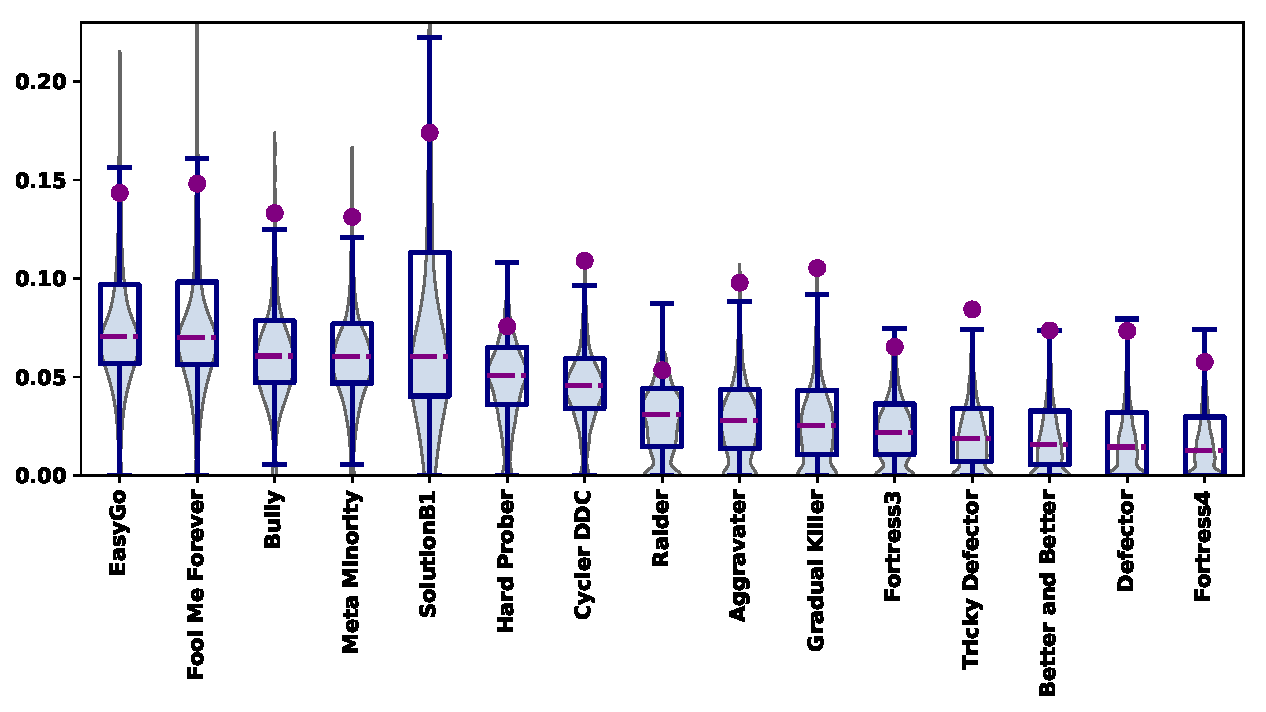
\includegraphics[width=.8\textwidth]{../images/performance_probend.pdf}
    \caption{\(\bar{r}\) distributions for best performed strategies in probabilistic ending tournaments.}
    \label{fig:probend_results}
\end{figure}

\subsection{Noisy \& probabilistic ending tournaments}\label{subsection:noisy_probend_tournament}

This section presents the results in tournaments were there are two
uncertainties. There is the uncertainty that a player's action will be flipped
and there is the uncertainty that there will not be future interactions.
The 15 top ranked strategies are given in Table~\ref{table:noisy_prob_end_results}.
Several of these strategies were highly ranked in noisy tournaments as well
but the same does not hold for the strategies which were highly ranked in
probabilistic ending tournaments.

\begin{table}[!htbp]
    \centering
    \resizebox{.28\textwidth}{!}{
    \begin{tabular}{lr}
\toprule
Name                &                         $\bar{r}$    \\
\midrule
Alternator          &                                 0.30390 \\
$\phi$              &                                 0.31025 \\
$e$                 &                                 0.31293 \\
$\pi$               &                                 0.31818 \\
Limited Retaliate   &                                 0.35294 \\
Anti Tit For Tat    &                                 0.35429 \\
Retaliate 3         &                                 0.35484 \\
Limited Retaliate 3 &                                 0.35563 \\
Retaliate           &                                 0.35588 \\
Retaliate 2         &                                 0.35714 \\
Limited Retaliate 2 &                                 0.36066 \\
Hopeless            &                                 0.36913 \\
Arrogant QLearner   &                                 0.40526 \\
Cautious QLearner   &                                 0.40711 \\
Risky QLearner      &                                 0.41989 \\
\bottomrule
\end{tabular}
}
    \caption{Noisy and probabilistic ending top performances}\label{table:noisy_prob_end_results}
\end{table}

The top ranked strategy is Alternator a strategy that alternate between
cooperation and defection. Alternator is followed by strategies that decide so
that the ratio of cooperations and defections is close to the equivalent
mathematical constants. Anti Tit For Tat is similar to Bully, which was covered
in Section~\ref{subsection:noisy_tournament}, but starts of with cooperation and
Hopeless~\cite{Van2015} a strategy that will only defect if and only if a mutual
cooperation. The last spots are occupied by strategies based on the Q learning
algorithm.

Compared to the distributions in noisy environments,
Section~\ref{subsection:noisy_tournament}, the distributions here are skewed
towards the middle, Figure~\ref{fig:noisy_probend_results}. The medians are
close to 0.5 which seems to indicate a less dominant performance of strategies
in this environment.

\begin{figure}[!htbp]
    \centering
    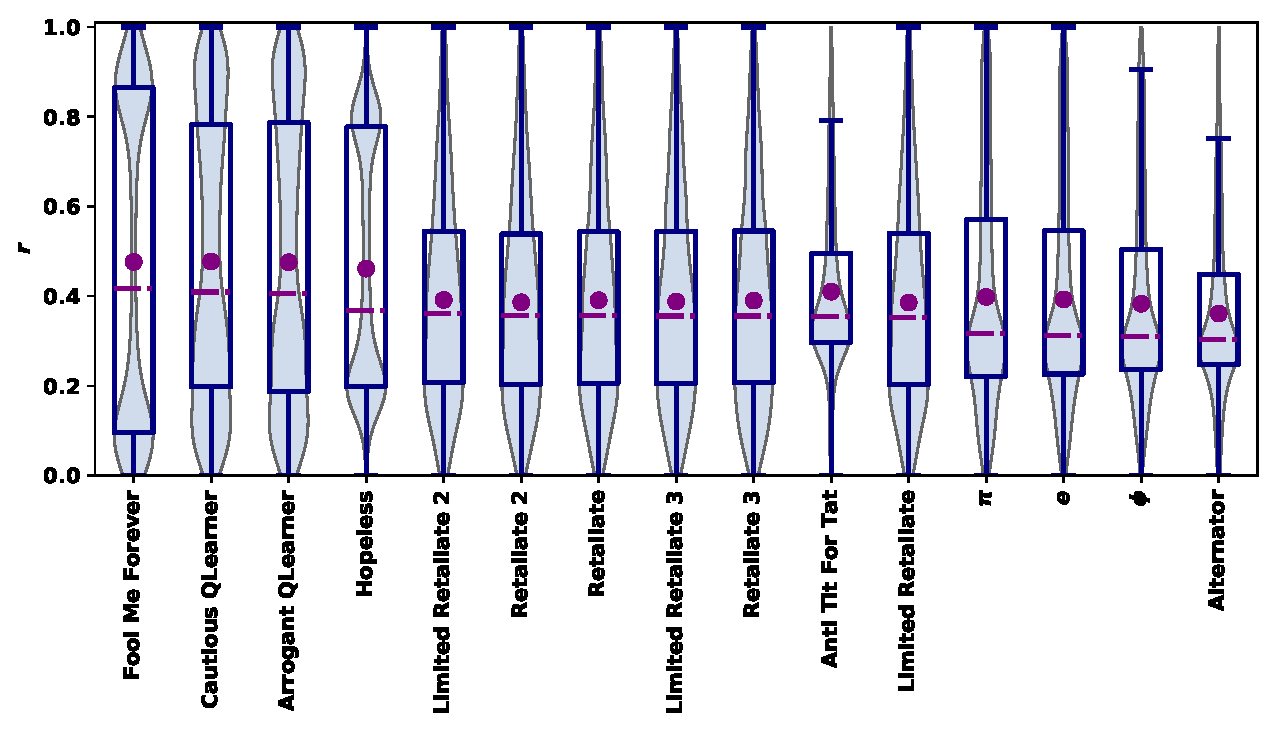
\includegraphics[width=.7\textwidth]{../images/performance_probend_noise.pdf}
    \caption{\(\bar{r}\) distributions for best performed strategies in noisy probabilistic ending tournaments.}
    \label{fig:noisy_probend_results}
\end{figure}

As yet, the performances of 186 different strategies have been evaluated in
four different tournaments. In standard tournaments the top ranked spots were
dominated by strategies that have been trained using reinforcement learning
techniques and have been maximised in a standard tournament against the same
list of opponents that is being used here. These strategies dominated most
the tournaments that have been involved in. In noisy tournaments the top ranked
strategies were all different to those of standard tournaments. Most of the
top ranked strategies have been strategies that were trying to keep the defection
and cooperation to a given ratio. These strategies had won most the tournaments
in which they participated, however, they also ranked last in several tournaments.
Once again in probabilistic ending tournaments the top ranked strategies were
different to those before. More defecting strategies occupied the top ranks
as well as finite state automata that have been introduced all by the same
authors. Finally, in noisy probabilistic ending tournaments it was the only
set of tournaments were the highly ranked strategies have been covered before,
more specifically, in noisy tournaments. In these tournaments however the
distributions of the ranks had much variation and some strategies even had
a $\bar{r}$ close to 0.5, indicating that there were successfully only 50\%
of the time.

In the following section the performance of the strategies is evaluated again.
However this time the results of the tournament types are included in the
analysis.

\subsection{Top performance in data set}\label{subsrction:overall}

The data set which was described in Section~\ref{section:data_collection}
contains results from 49,140 tournaments. The strategies have been ranked based
on their $\bar{r}$ and the 15 top ranked strategies are given in
Table~\ref{table:overall_results}. These include several strategies that have
ranked in the top spots in the separate tournament analysis. The top 6 spaces
are overtaken by Retaliate strategies, followed by BackStabber and
DoubleCrosser. DoubleCrosser is just an extension of BackStabber. Nice Meta
Winner and NMWE Memory One are strategies that are part of a team, Stein and
Rapoport and Grudger are strategies from Axelrod's original tournament that came
the 6th and 7th respectively. Forgeful Fool Me once is an extension to Grudger
and PSO GAmer and Evolved are strategies again introduced in~\cite{Harper2017}.

\begin{table}[!htbp]
    \centering
    \resizebox{.35\textwidth}{!}{
    \begin{tabular}{lr}
\toprule
{} &  Normalized\_Rank \\
Name                    &                  \\
\midrule
Evolved FSM 16          &            0.018 \\
Evolved HMM 5           &            0.019 \\
Evolved FSM 16 Noise 05 &            0.025 \\
EvolvedLookerUp2\_2\_2    &            0.028 \\
Evolved ANN             &            0.037 \\
PSO Gambler 2\_2\_2       &            0.040 \\
Evolved ANN 5           &            0.046 \\
PSO Gambler 1\_1\_1       &            0.061 \\
Fool Me Once            &            0.067 \\
Evolved FSM 4           &            0.075 \\
DoubleCrosser           &            0.079 \\
Winner12                &            0.081 \\
BackStabber             &            0.082 \\
DBS                     &            0.086 \\
PSO Gambler Mem1        &            0.089 \\
\bottomrule
\end{tabular}
}
    \caption{Top performances in data set}\label{table:overall_results}
\end{table}

The distributions between the first six strategies are very similar. From then
onwards the distributions are skewed to both 0 and 1. The analysis
of the data set gives us an indication of what performance is successful
in cases that the environment is not known to you and the Retaliate family
seem to be doing the trick.

\begin{figure}[!htbp]
    \centering
    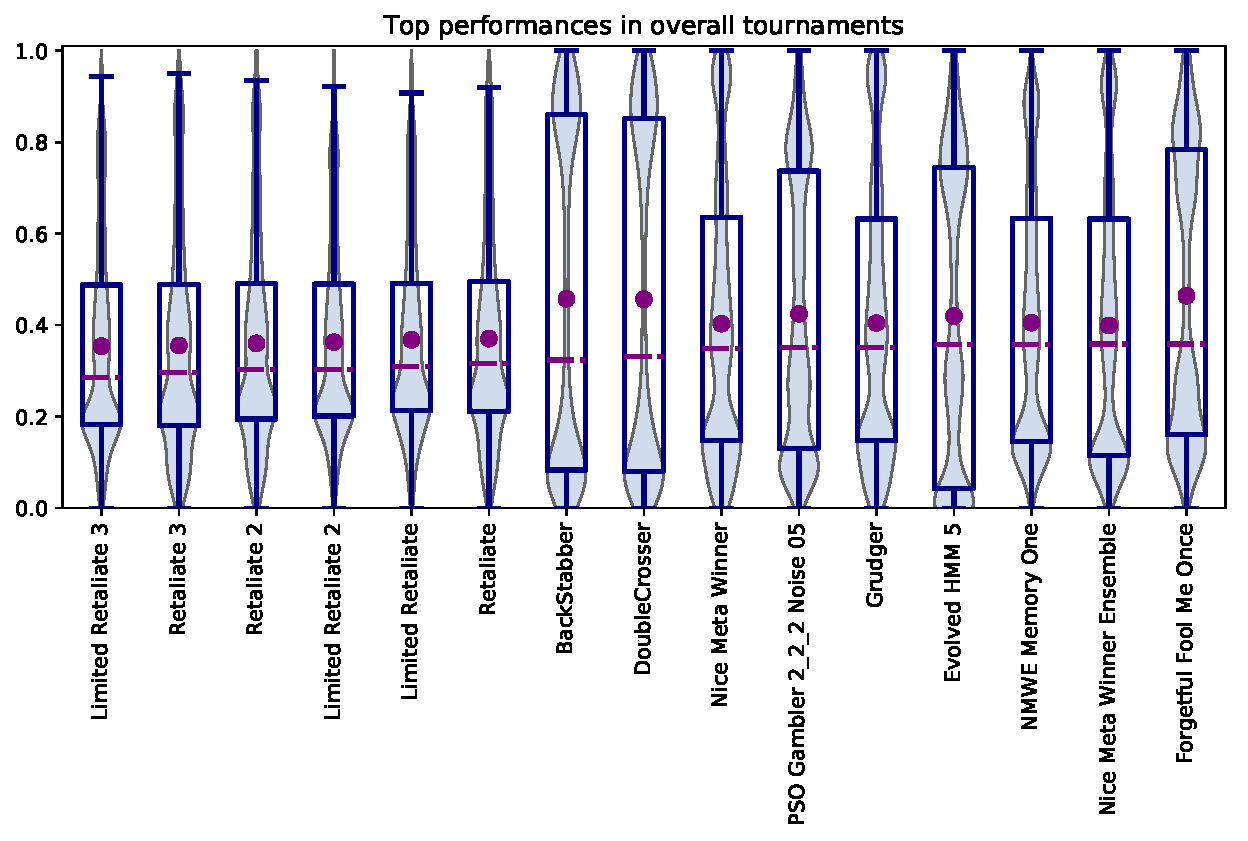
\includegraphics[width=.8\textwidth]{../images/performance_merged.pdf}
    \caption{\(\bar{r}\) distributions for best performed strategies in data set.}
    \label{fig:overall_results}
\end{figure}

In this section the top ranked performances were presented. These one done
just by simply taking into account the ranks each strategy achieved in each
tournament type and finally in the data set. Through the analysis only a few
strategies seem to have been repeated, however, the winner were also
completely different from type to type. Thus, what does make then successfully
in those environments? The aim of the next section is that.

\section{Evaluation of performance}\label{section:evaluation_of_performance}

In this section we evaluate what makes a strategy.


% \begin{figure}
%     \centering
%     \includegraphics[width=.7\textwidth]{../output/output/standard/feature_importance_bar_plot.pdf}
% \end{figure}

\section{Conclusion and Discussion}\label{section:conclusion}

\bibliographystyle{plain}
\bibliography{bibliography}
\end{document}